\chapter{THIẾT KẾ VÀ THỰC HIỆN PHẦN MỀM NHÚNG CHO LOGIC ANALYZER}

\section{Yêu cầu thiết kế}
Các yêu cầu thiết kế chính cho phần mềm nhúng trên Logic analyzer bao gồm:
\begin{itemize}
    \item Có khả năng giao tiếp USB với máy tính để nhận lệnh cấu hình và điều khiển.
    \item Có khả năng thu thập các tín hiệu số và tín hiệu tương tự từ DUT.
    \item Có tích hợp UART hỗ trợ debug.
\end{itemize}

\section{State machine tổng quát của Logic analyzer}
\begin{figure}[H]
    \centering
    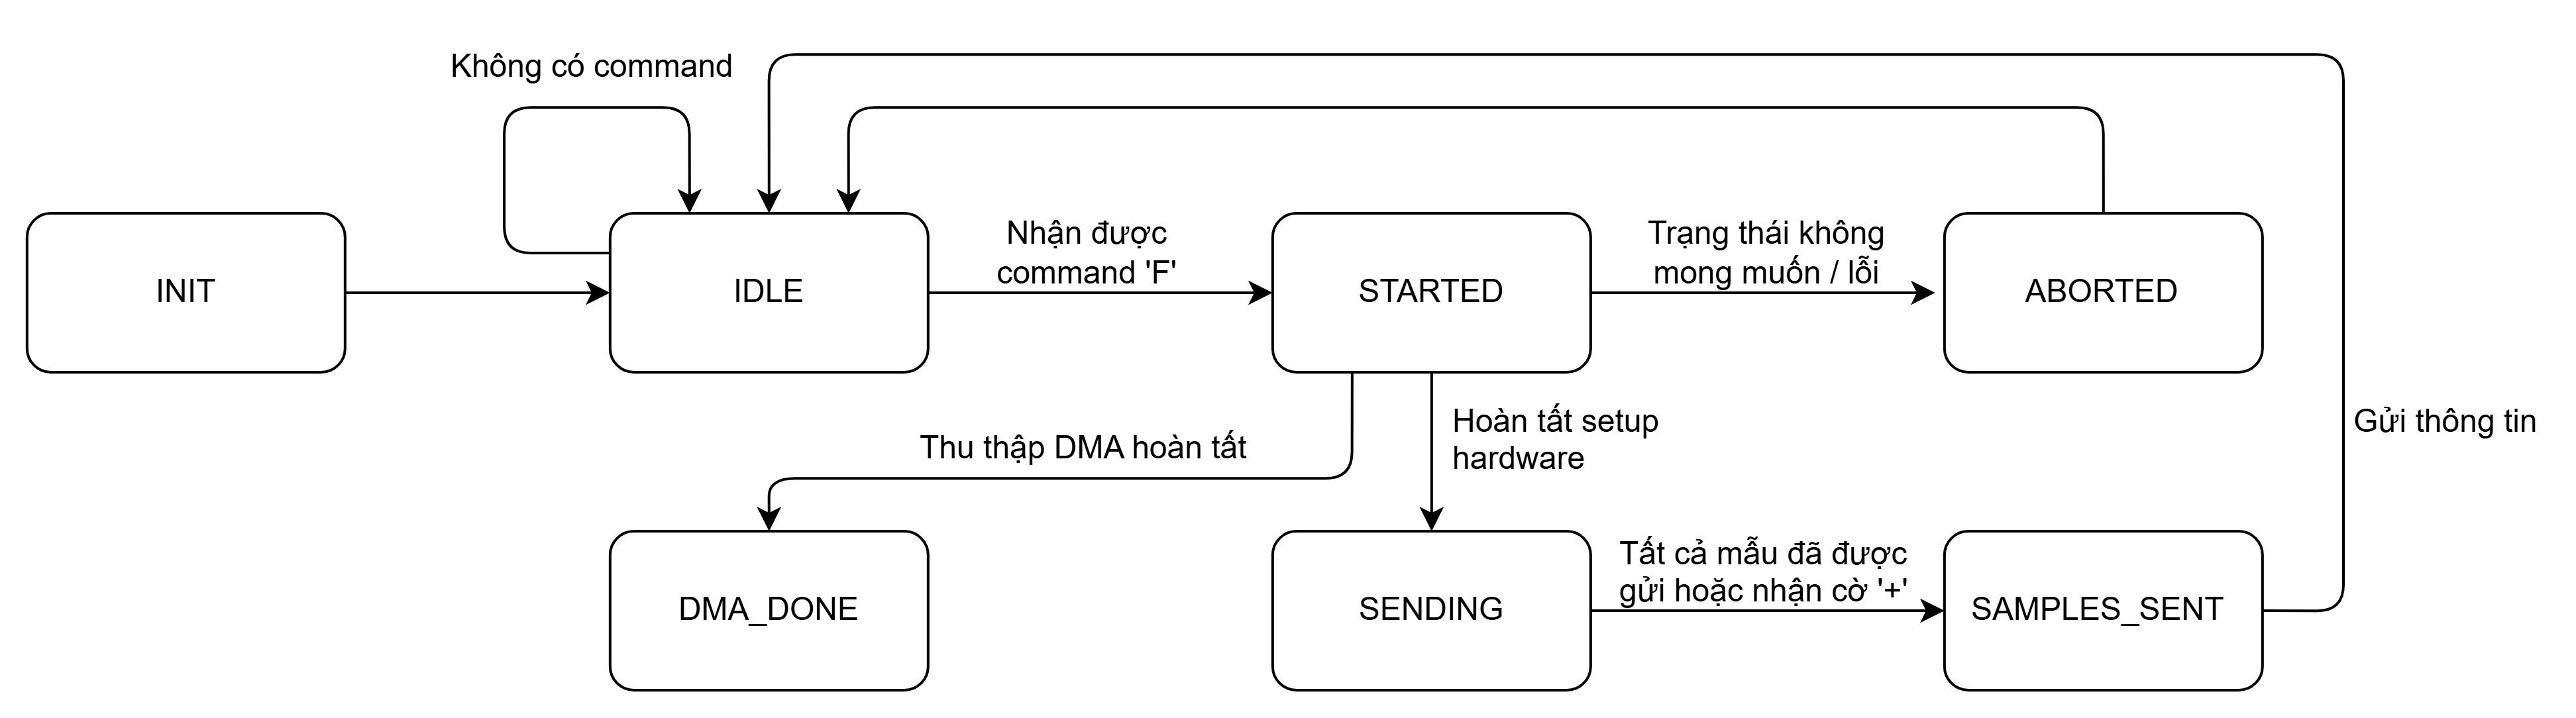
\includegraphics[width=1\textwidth]{image/LA_state_machine.jpg}
    \caption{State machine của Logic analyzer}
    \label{fig:LA_state_machine}
\end{figure}

Các trạng thái chính của Logic analyzer gồm:
\begin{itemize}
    \item \textbf{INIT}: Trạng thái khởi tạo hệ thống, cấu hình các ngoại vi và chuẩn bị cho việc thu thập dữ liệu.
    \item \textbf{IDLE}: Trạng thái chờ lệnh từ máy tính.
    \item \textbf{STARTED}: Trạng thái bắt đầu thu thập dữ liệu.
    \item \textbf{SENDING}: Trạng thái gửi dữ liệu đã thu thập cho máy tính.
    \item \textbf{DMA\_DONE}: Trạng thái hoàn thành thu thập dữ liệu bằng DMA.
    \item \textbf{ABORTED}: Trạng thái hủy bỏ quá trình thu thập dữ liệu do lỗi.
    \item \textbf{SAMPLES\_SENT}: Trạng thái hoàn thành việc gửi dữ liệu.
\end{itemize}

\section{Lưu đồ giải thuật chi tiết của Logic analyzer}
\subsection{Lưu đồ giải thuật của Logic analyzer}
\begin{figure}[H]
    \centering
    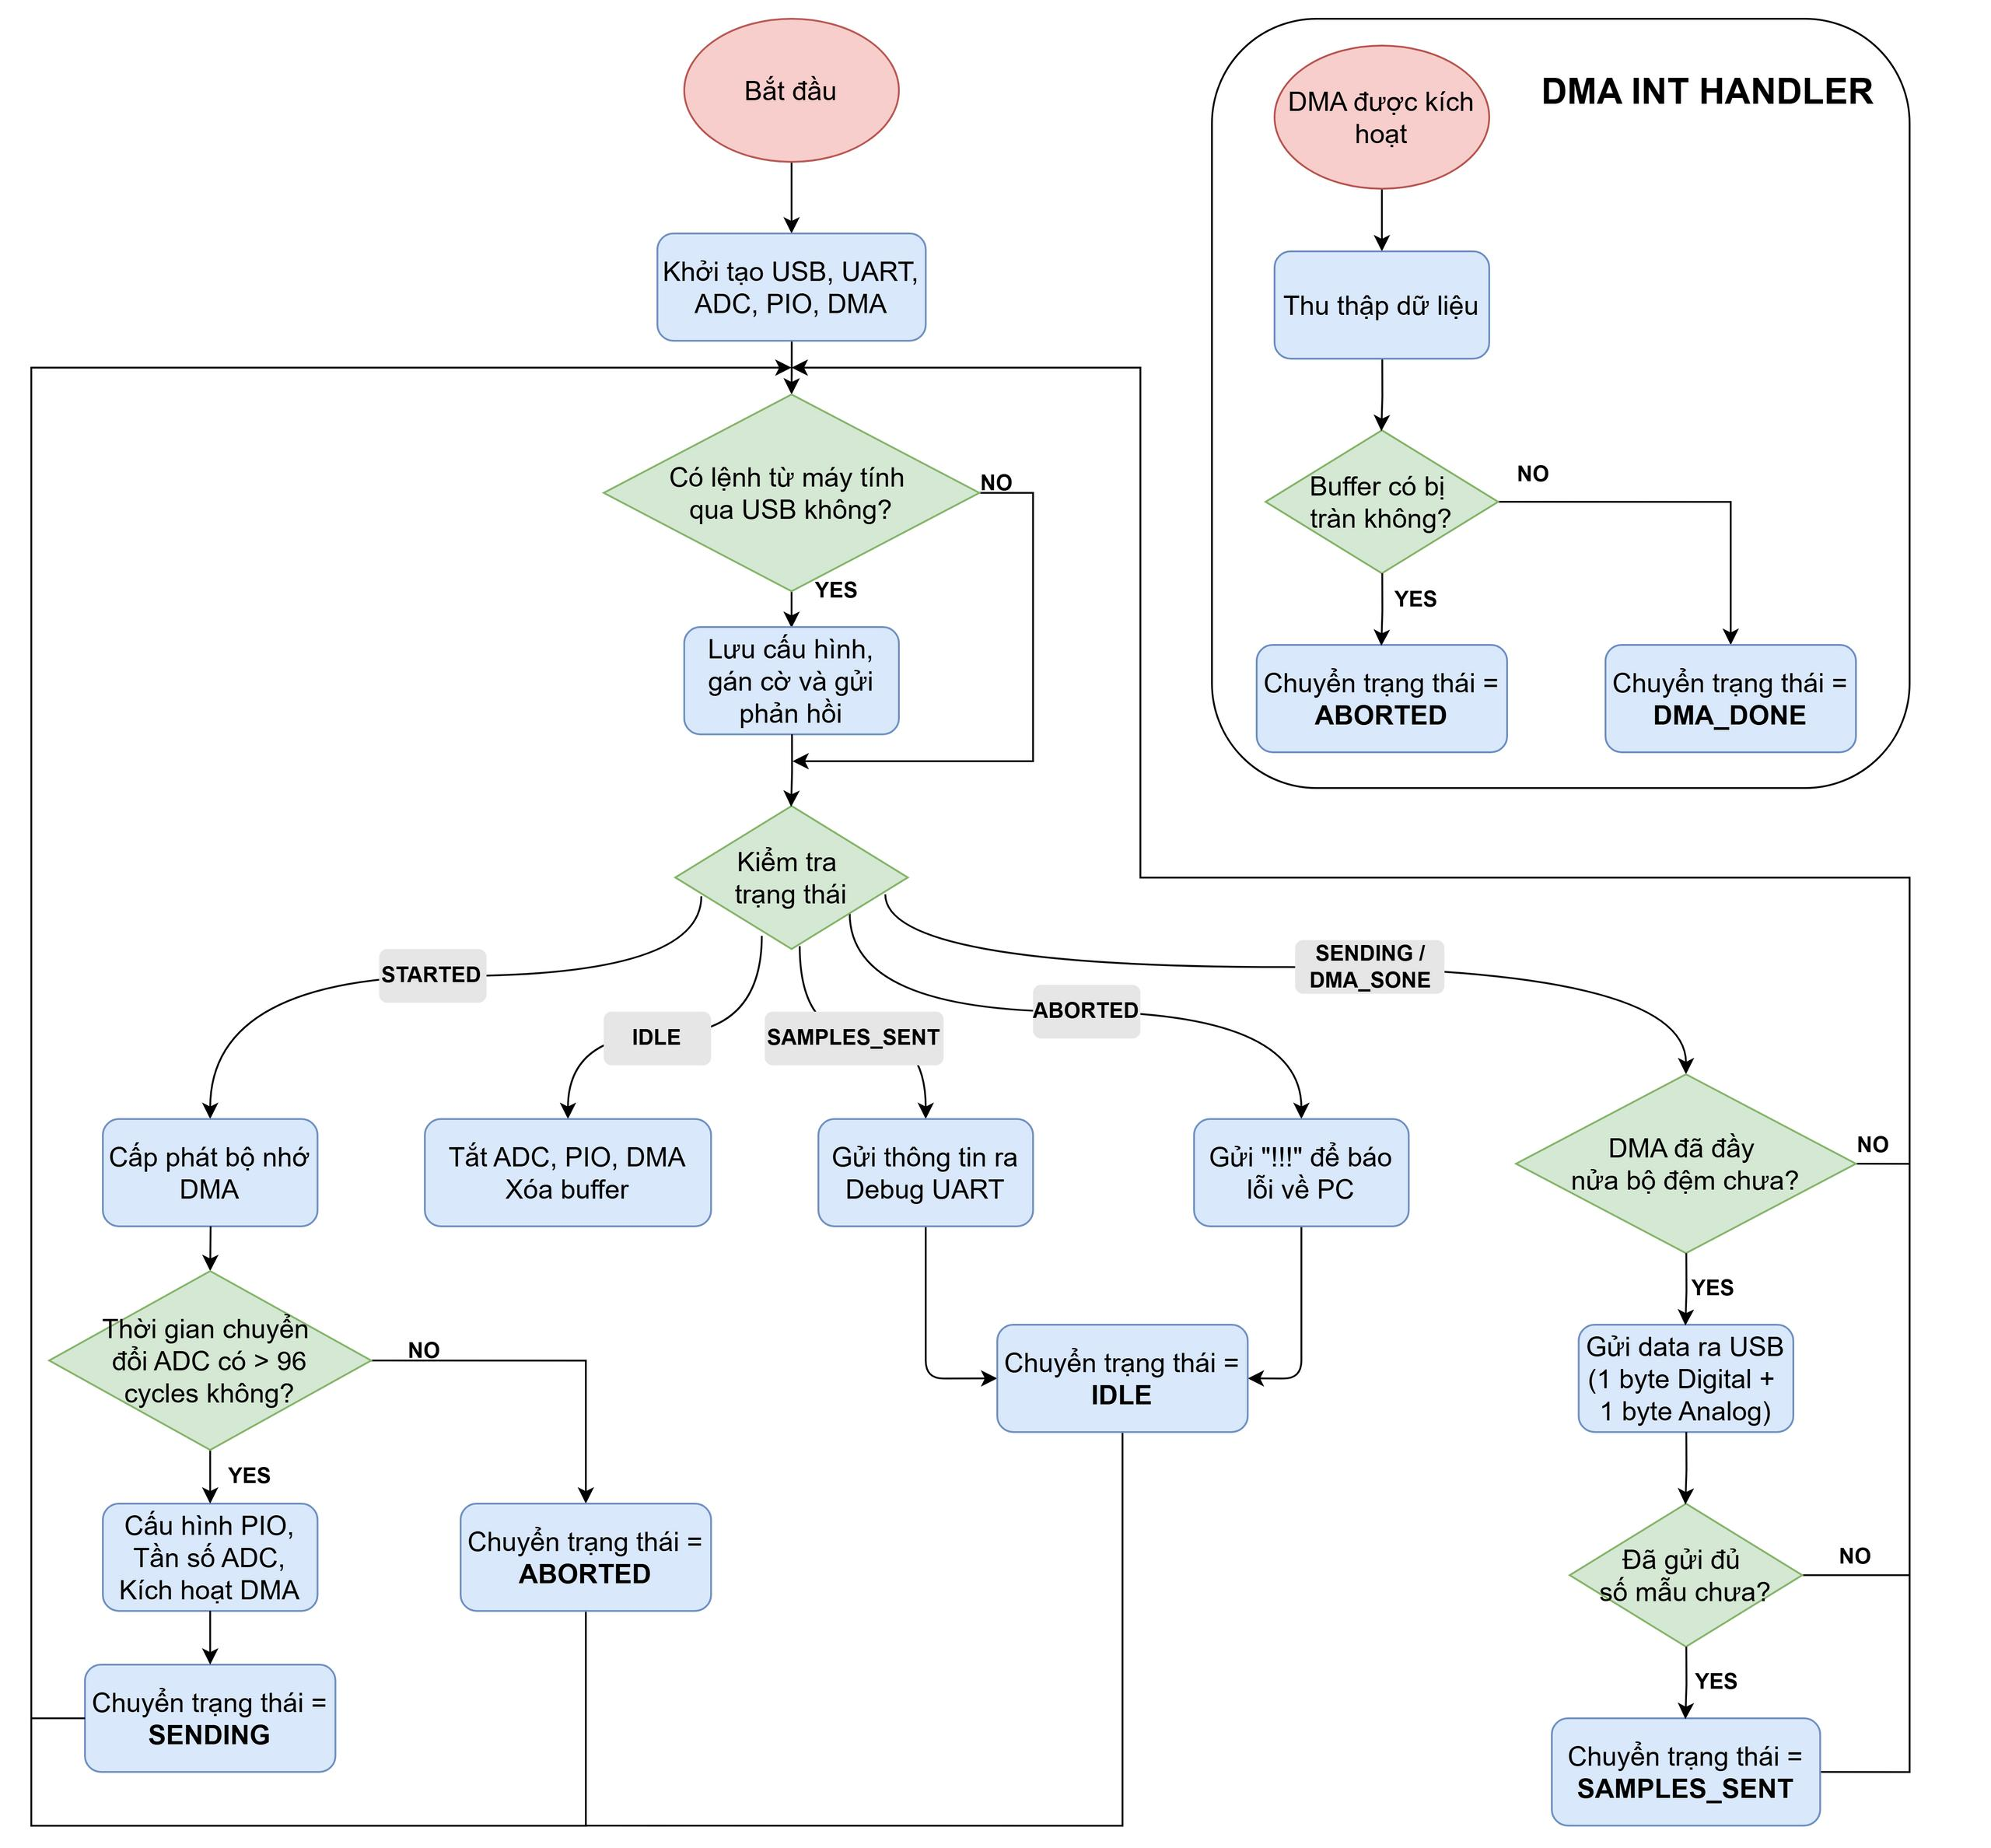
\includegraphics[width=1\textwidth]{image/LA_flow_chart.jpg}
    \caption{Lưu đồ giải thuật của Logic analyzer}
    \label{fig:LA_flow_chart}
\end{figure}

Logic analyzer hoạt động trong một vòng lặp vô hạn kết hợp với ngắt DMA nhằm tối ưu hóa tốc độ cho quá trình thu thập và truyền dữ liệu.
Quá trình bắt đầu bằng việc khởi tạo các ngoại vi cần thiết như USB, UART, ADC, PIO và DMA. Sau khi khởi tạo hoàn tất, hệ thống chuyển sang trạng thái IDLE để chờ lệnh từ máy tính.

Khi nhận được các lệnh từ máy tính, Logic analyzer sẽ lưu cấu hình, gán cờ và gửi phản hồi về máy tính. Nếu nhận được lệnh 'F', Logic analyzer sẽ chuyển sang trạng thái STARTED và thực hiện cấp phát bộ nhớ cho DMA.
Sau đó nếu tính toán nếu thời gian chuyển đổi của ADC lớn hơn 96 cycles, Logic analyzer sẽ tiếp tục cấu hình các ngoại vi khác, kích hoạt DMA và chuyển sang trạng thái SENDING.
Ngược lại, Logic analzyer sẽ chuyển sang trạng thái ABORTED do thời gian chuyển đổi của ADC trên Raspberry Pi tối thiểu là 96 cycles, nếu lấy mẫu với tốc độ quá lớn sẽ dẫn đến các lỗi không mong muốn.

Quá trình gửi và thu thập dữ liệu được thực hiện song song thông qua ngắt DMA (DMA Interrupt Handler). Khi DMA được kích hoạt, dữ liệu sẽ được ghi vào bộ đệm.
Logic analyzer sẽ kiểm tra tình trạng bộ đệm. Nếu không gửi kịp dữ liệu lên máy tính, bộ đệm sẽ bị tràn và hệ thống sẽ chuyển sang trạng thái ABORTED.
Ngược lại, nếu thu thập đủ dữ liệu, Logic analyzer sẽ chuyển sang trạng thái DMA\_DONE.

Trong trạng thái SENDING / DMA\_DONE, Logic analyzer sẽ kiểm tra buffer đã đầy một nửa hay chưa để thực hiện cơ chế truyền dữ liệu theo từng phần.
Dữ liệu sau đó được gửi ra máy tính qua USB, với định dạng mỗi mẫu gồm 1 byte tín hiệu số và 1 byte tín hiệu tương tự. Quá trình này lặp lại cho đến khi toàn bộ số mẫu đã được truyền đi.
Khi đã gửi đủ số mẫu, Logic analyzer sẽ chuyển sang trạng thái SAMPLES\_SENT và tắt ADC, PIO, DMA, xóa bộ đệm để sẵn sàng cho chu kỳ thu thập tiếp theo.

\subsection{Cơ chế xử lý bộ đệm DMA}
\begin{figure}[H]
    \centering
    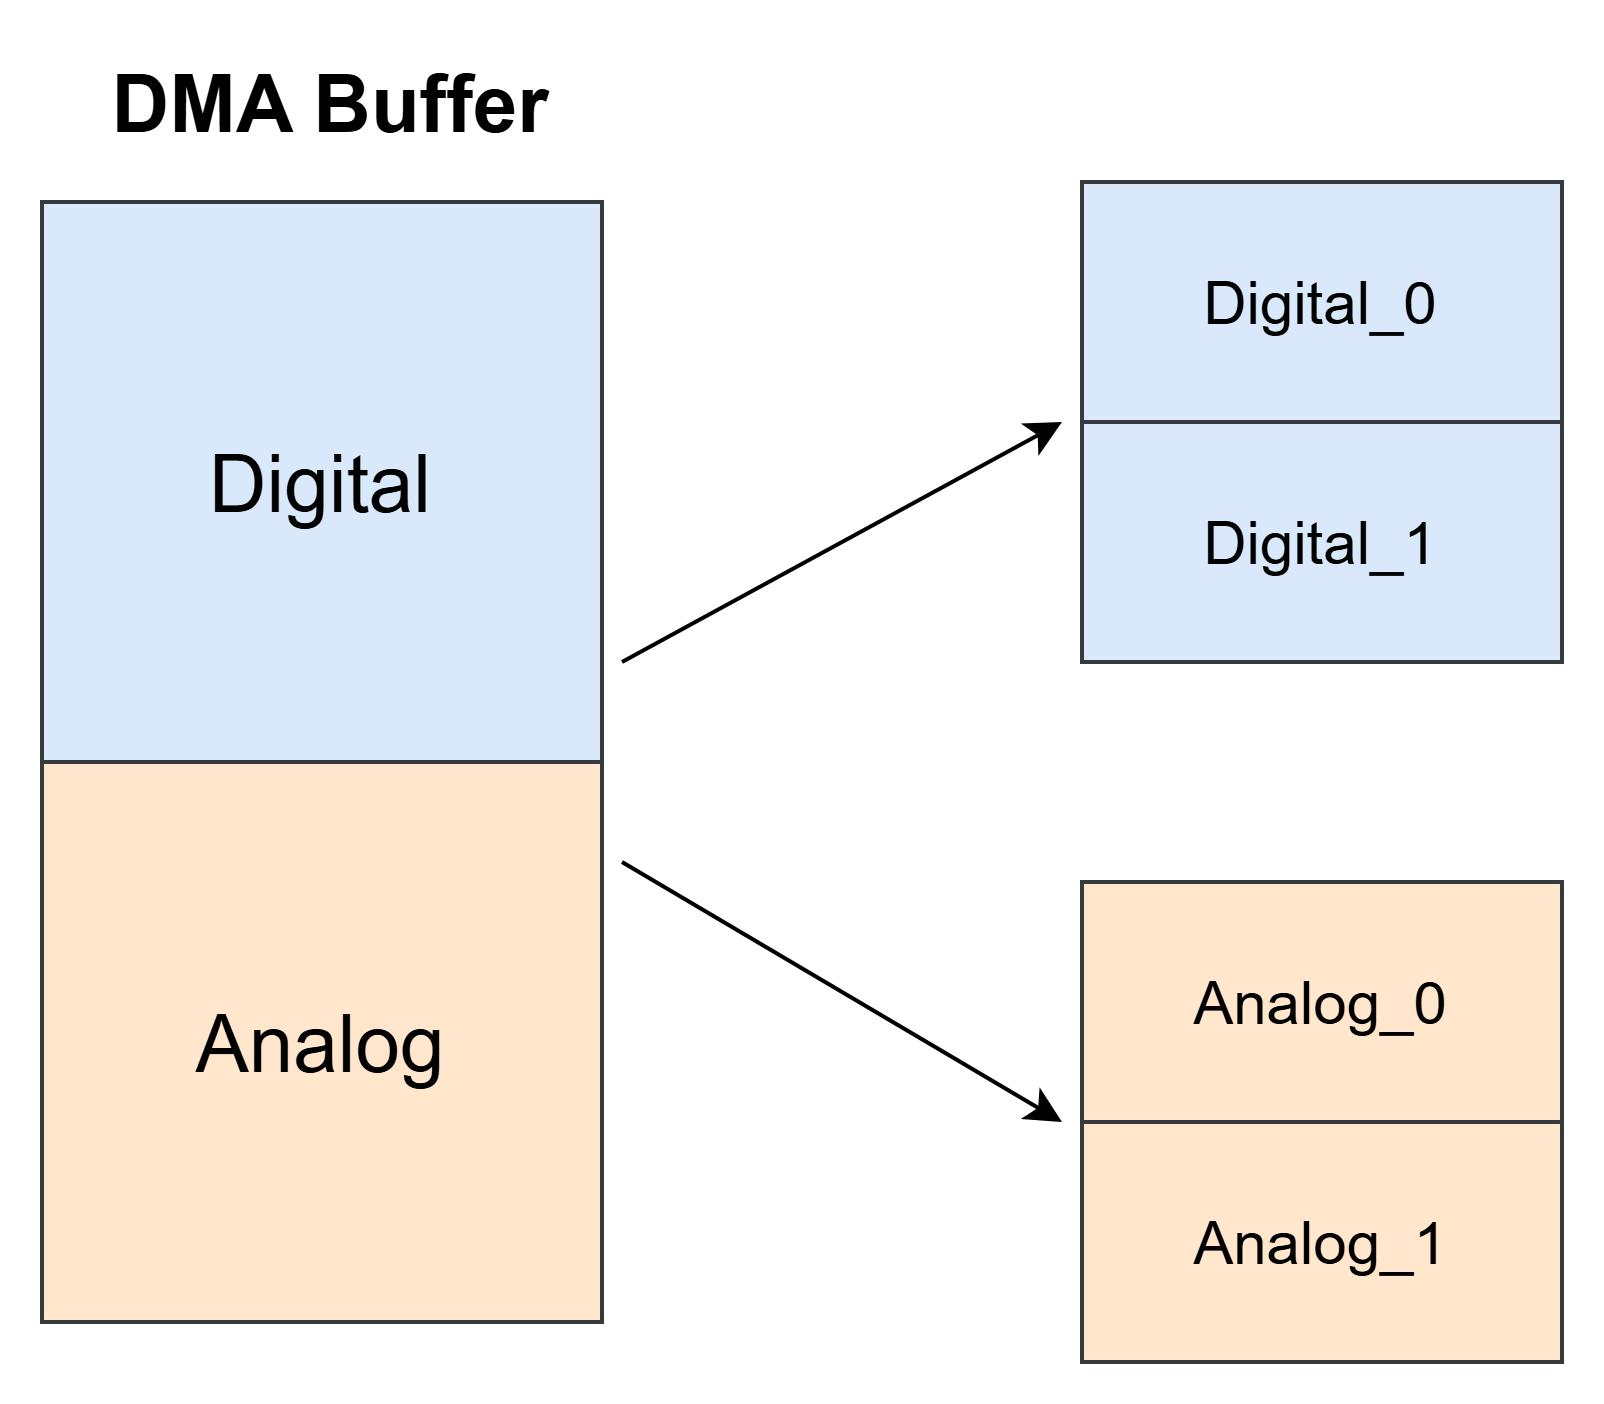
\includegraphics[width=0.5\textwidth]{image/LA_dma_buffer.jpg}
    \caption{Cấp phát bộ đệm DMA}
    \label{fig:LA_dma_buffer}
\end{figure}
